\section{Green MGGP: Formulation and Theory}\label{sec:method}

This section formalises the model class, the multigene representation and the two objectives, establishes the
properties on which Green MGGP relies, and characterises both the lexicographic scheme of the package and the
proposed Pareto-based scheme. The main symbols are collected in Table~\ref{tab:symbols}, and
Fig.~\ref{fig:pipeline} gives an overview of the method, from the data to the execution of the selected model,
marking the components to which each theoretical result applies.

\begin{figure}[t]
\centering
\resizebox{\textwidth}{!}{% Methodology pipeline of Green MGGP (TikZ). Included by sec_method.tex; needs
% \usepackage{tikz} and \usetikzlibrary{arrows.meta,calc}. Designed at 16 cm width.
\begin{tikzpicture}[
  x=1cm, y=1cm, line cap=round,
  font=\fontsize{6.4}{7.4}\selectfont,
  >={Stealth[length=3.6pt,width=3pt]},
  stage/.style={draw=black!16, fill=black!2.5, rounded corners=4pt, line width=0.5pt},
  head/.style={rounded corners=4pt, text=white, font=\fontsize{7.2}{8}\selectfont\bfseries,
               minimum height=0.44cm, inner sep=2pt, anchor=north west},
  box/.style={draw=#1, fill=#1!8, rounded corners=2.5pt, line width=0.6pt, align=center, inner sep=2.4pt},
  box/.default=black,
  gbox/.style={draw=black!45, fill=black!5, rounded corners=2.5pt, line width=0.6pt, align=center, inner sep=2.4pt},
  lbl/.style={font=\fontsize{5.6}{6.5}\selectfont, text=black!62, align=center},
  flow/.style={->, line width=0.7pt, draw=black!72},
  thin/.style={->, line width=0.5pt, draw=black!50},
  badge/.style={draw=black!30, fill=white, rounded corners=5pt, align=center, inner sep=2.4pt,
                font=\fontsize{5.6}{6.6}\selectfont, text width=#1},
  badge/.default=2.6cm,
  tag/.style={circle, fill=cInk, text=white, font=\fontsize{5}{5}\selectfont\bfseries, inner sep=0pt,
              minimum size=8pt},
]
\definecolor{cData}{HTML}{0072B2}
\definecolor{cGreen}{HTML}{009E73}
\definecolor{cLex}{HTML}{E69F00}
\definecolor{cCost}{HTML}{D55E00}
\definecolor{cExec}{HTML}{CC79A7}
\definecolor{cInk}{HTML}{263238}
\def\sub{\fontsize{5.6}{6.5}\selectfont\color{black!62}}

% ================================================================= stage frames
\draw[stage] (0,1.9) rectangle (2.6,9.1);
\draw[stage] (2.75,1.9) rectangle (10.25,9.1);
\draw[stage] (10.4,1.9) rectangle (13.0,9.1);
\draw[stage] (13.15,1.9) rectangle (16,9.1);
\node[head, fill=cData,  minimum width=2.6cm]  at (0,9.1)     {1\quad data};
\node[head, fill=cGreen, minimum width=7.5cm]  at (2.75,9.1)  {2\quad multigene GP search under the cost $C_\rho$};
\node[head, fill=cInk,   minimum width=2.6cm]  at (10.4,9.1)  {3\quad trade-off set};
\node[head, fill=cExec,  minimum width=2.85cm] at (13.15,9.1) {4\quad execution};

% ================================================================= 1  DATA
\node[box=cData, minimum width=1.05cm, minimum height=0.5cm] (plant) at (1.38,7.7) {plant\\[-1pt]\sub E1, E2, E3};
\draw[thin] (0.1,7.7) -- node[above, lbl, pos=0.5, yshift=-1pt]{$u(k)$} (plant.west);
\node[draw=black!50, circle, inner sep=0.5pt, font=\fontsize{5.5}{5}\selectfont] (sum) at (2.3,7.7) {$+$};
\draw[thin] (plant.east) -- (sum.west);
\draw[thin] (2.3,8.2) node[above, lbl, yshift=-2.5pt]{$e(k)$} -- (sum.north);
\draw[thin] (sum.south) -- (2.3,7.25) node[below, lbl, yshift=1pt]{$y(k)$};
\begin{scope}[shift={(0.18,5.85)}]
  \draw[black!25, line width=0.35pt] (0,0) -- (2.15,0);
  \draw[cData, line width=0.6pt, domain=0:2.05, samples=70, smooth]
     plot (\x, {0.3*sin(deg(3.6*\x)) + 0.08*sin(deg(10.8*\x)) + 0.78});
  \draw[black!80, line width=0.6pt, domain=0:2.05, samples=70, smooth]
     plot (\x, {0.24*sin(deg(3.6*\x - 0.6)) + 0.27});
  \node[lbl, anchor=west] at (2.08,0.8) {$u$};
  \node[lbl, anchor=west] at (2.08,0.27) {$y$};
  \node[lbl] at (1.07,-0.2) {E1, E2: bilinear};
\end{scope}
\begin{scope}[shift={(1.3,4.55)}]
  \draw[->, black!35, line width=0.35pt] (-0.85,0) -- (0.85,0) node[right, lbl, xshift=-2pt]{$u$};
  \draw[->, black!35, line width=0.35pt] (0,-0.52) -- (0,0.58) node[above, lbl, yshift=-3pt]{$y$};
  \draw[black!80, line width=0.6pt, smooth cycle, tension=0.85]
    plot coordinates {(-0.7,-0.4) (-0.18,-0.28) (0.4,0.06) (0.7,0.4) (0.18,0.28) (-0.4,-0.06)};
  \node[lbl] at (0,-0.72) {E3: Bouc--Wen};
\end{scope}
\fill[cData!75] (0.18,3.12) rectangle (1.75,3.4);
\fill[cData!25] (1.75,3.12) rectangle (2.42,3.4);
\node[font=\fontsize{5.3}{6}\selectfont\bfseries, text=white] at (0.965,3.26) {identification};
\node[font=\fontsize{5.3}{6}\selectfont, text=cData] at (2.085,3.26) {val.};
\node[lbl, anchor=north] at (1.3,3.08) {E1/E2: $70\%$ / $30\%$};
\node[lbl, align=center, anchor=north, text width=2.35cm] at (1.3,2.7)
  {$J_E$ and $\mathcal M_\tau$ use identification data only};

% ================================================================= 2  SEARCH
\foreach \o/\op in {0.22/0.3, 0.11/0.55, 0/1} {
  \draw[draw=cGreen!65!black, fill=white, fill opacity=\op, rounded corners=2pt, line width=0.5pt]
     (2.95+\o,5.25+\o) rectangle (4.4+\o,7.95+\o);
}
\node[font=\fontsize{6.4}{7}\selectfont\bfseries, text=cGreen!55!black] at (3.675,7.7) {population};
\node[lbl] at (3.675,7.45) {$P_t$,\; $\mu=100$};
\foreach \gx/\gc in {3.255/cCost, 3.675/cData, 4.095/cExec} {
  \draw[\gc, line width=0.45pt] (\gx,7.0) -- (\gx-0.13,6.72) (\gx,7.0) -- (\gx+0.13,6.72) (\gx-0.13,6.72) -- (\gx-0.13,6.45);
  \foreach \p in {(\gx,7.0),(\gx-0.13,6.72),(\gx+0.13,6.72),(\gx-0.13,6.45)} \fill[\gc] \p circle (1.25pt);
}
\node[lbl, font=\fontsize{5.1}{6}\selectfont] at (3.675,6.12) {$\mathbf M$: $G$ genes};
\node[lbl, font=\fontsize{5.1}{6}\selectfont] at (3.675,5.85) {\texttt{mul}, $q_j$, $y_1$, $u_1$};
\node[gbox, text width=1.45cm, font=\fontsize{5.6}{6.5}\selectfont] (var) at (3.675,4.55)
  {crossover,\\ mutation $\to Q_t$};
\draw[thin] (var.north) -- (3.675,5.25);
\draw[thin] (2.6,7.05) -- (2.95,7.05);

% evaluation column
\def\ex{5.95}
\node[box=cGreen, text width=2.35cm] (kappa) at (\ex,7.8)
  {$\kappa$: gene $\to$ monomial\\[-0.5pt]\sub structure $\mathcal R(\mathbf M)$};
\node[box=cGreen, text width=2.35cm] (ls) at (\ex,6.95)
  {least squares\\[-0.5pt]\sub $\Psi=\bar\Psi A$,\; unique $\bar{\boldsymbol\theta}^\star$};
\node[box=cGreen, text width=2.35cm] (je) at (\ex,6.1)
  {error $J_E$\\[-0.5pt]\sub multiple shooting};
\begin{scope}[shift={(\ex-0.83,5.42)}]
  \foreach \w in {0,0.57,1.14} {
    \draw[black!28, line width=0.35pt] (\w,0) rectangle (\w+0.5,0.17);
    \draw[cGreen!75!black, line width=0.45pt] (\w,0.04) .. controls (\w+0.18,0.17) and (\w+0.32,0.01) .. (\w+0.5,0.13);
  }
\end{scope}
\node[box=cCost, text width=2.35cm] (cost) at (\ex,4.5)
  {cost $C_\rho=a+\rho\,b$\\[-0.5pt]\sub $a$ additions, $b$ multiplications};
\draw[flow] (4.4,7.8) -- (kappa.west);
\draw[thin] (kappa) -- (ls);
\draw[thin] (ls) -- (je);
\draw[thin] (\ex,5.4) -- (cost.north);
\node[lbl, anchor=north] at (\ex,4.0) {objectives $\mathbf F=(J_E,\,C_\rho)$};

% selection column
\def\sx{8.75}
\node[box=cGreen, text width=2.65cm, minimum height=3.35cm] (green) at (\sx,6.45) {};
\node[font=\fontsize{6.4}{7}\selectfont\bfseries, text=cGreen!55!black] at (\sx,7.88) {Green MGGP};
\begin{scope}[shift={(\sx-0.95,6.1)}]
  \draw[->, black!40, line width=0.35pt] (0,0) -- (1.9,0) node[right, lbl, xshift=-1pt]{$C_\rho$};
  \draw[->, black!40, line width=0.35pt] (0,0) -- (0,1.45) node[left, lbl, yshift=-3pt]{$J_E$};
  \draw[cGreen!35, line width=0.5pt, densely dashed] (0.32,1.32) -- (0.32,0.97) -- (0.78,0.97) -- (0.78,0.72) -- (1.3,0.72) -- (1.3,0.52) -- (1.75,0.52);
  \draw[cGreen!80!black, line width=0.55pt] (0.14,1.25) -- (0.14,0.72) -- (0.5,0.72) -- (0.5,0.44) -- (1.0,0.44) -- (1.0,0.25) -- (1.7,0.25);
  \foreach \p in {(0.32,0.97),(0.78,0.72),(1.3,0.52)} \fill[cGreen!35] \p circle (1.15pt);
  \foreach \p in {(0.14,0.72),(0.5,0.44),(1.0,0.25),(1.7,0.25)} \fill[cGreen!80!black] \p circle (1.25pt);
  \node[lbl, anchor=west] at (1.05,0.4) {$\mathcal F_1$};
  \node[lbl, anchor=west] at (1.33,0.85) {$\mathcal F_2$};
\end{scope}
\node[lbl] at (\sx,5.72) {rank $+$ crowding $\delta$};
\node[draw=cGreen, fill=white, rounded corners=2pt, line width=0.5pt, text width=2.35cm, align=center,
      inner sep=2.2pt, font=\fontsize{5.6}{6.5}\selectfont] (surv) at (\sx,5.18)
  {$U_t$: distinct $P_t\cup Q_t$\\ NSGA-II survival};
\node[box=cLex, text width=2.65cm, dashed, text=black!72] (lex) at (\sx,3.95)
  {MO-lex (baseline)\\[-0.5pt]\sub $J_E$ first; $C_\rho$ only breaks ties};
\draw[flow] (cost.east) -- (7.3,4.5) |- (green.west);
\draw[thin, cLex, densely dashed] (7.3,4.5) |- (lex.west);
% generation loop above the evaluation column
\draw[flow, cGreen!70!black, rounded corners=3pt] (green.north) -- (\sx,8.5) -- (3.9,8.5) -- (3.9,8.17);
\node[font=\fontsize{5.6}{6.5}\selectfont, text=cGreen!55!black, fill=black!2.5, inner sep=1pt] at (5.6,8.5)
  {next generation $t\to t+1$,\; $T=50$};

% ================================================================= 3  TRADE-OFF SET
\begin{scope}[shift={(10.75,5.45)}]
  \fill[cGreen!12] (0.16,2.45) -- (0.16,1.3) -- (0.5,1.3) -- (0.5,0.88) -- (0.88,0.88) -- (0.88,0.55) -- (1.42,0.55) -- (1.42,0.38) -- (1.95,0.38) -- (1.95,2.45) -- cycle;
  \draw[->, black!55, line width=0.45pt] (0,0) -- (2.1,0);
  \node[lbl, anchor=south east, inner sep=1pt] at (2.12,0.04) {$C_\rho/C_\mathrm{ref}$};
  \draw[->, black!55, line width=0.45pt] (0,0) -- (0,2.65) node[left, lbl, yshift=-3pt]{$J_E$};
  \draw[cGreen!80!black, line width=0.65pt] (0.16,2.45) -- (0.16,1.3) -- (0.5,1.3) -- (0.5,0.88) -- (0.88,0.88) -- (0.88,0.55) -- (1.42,0.55) -- (1.42,0.38) -- (1.95,0.38);
  \foreach \p in {(0.16,1.3),(0.5,0.88),(0.88,0.55),(1.42,0.38)} \fill[cGreen!80!black] \p circle (1.45pt);
  \fill[black!70] (1.95,2.45) circle (1.3pt);
  \node[lbl, anchor=south east] at (2.0,2.48) {$\mathbf r=(1,1)$};
  \node[lbl] at (1.28,1.65) {hypervolume};
  \draw[cCost, densely dashed, line width=0.5pt] (0,0.63) -- (2.05,0.63);
  \draw[cCost, densely dashed, line width=0.5pt] (0.02,-0.3) -- (0.3,-0.3);
  \node[lbl, text=cCost, anchor=west, inner sep=1pt] at (0.32,-0.3) {$(1{+}\tau)J^{\min}$};
  \draw[cCost, line width=0.8pt] (0.88,0.55) circle (3.3pt);
  \node[lbl, text=cCost, anchor=east] at (0.8,0.45) {$\mathcal M_\tau$};
\end{scope}
\draw[flow] (green.east) -- ++(0.15,0) |- (10.75,6.6);
\node[lbl, text width=2.45cm] at (11.7,4.55) {returned set $\ND(P_T)$:\\ $\HV_\mathrm{id}$, $\HV_\mathrm{val}$, attainment};
\node[box=cCost, text width=2.25cm] (taurule) at (11.7,3.25)
  {$\tau$-rule\\[-0.5pt]\sub cheapest within $5\%$ of best $J_E$};

% ================================================================= 4  EXECUTION
\def\qx{14.575}
\node[lbl] at (\qx,8.4) {canonical simulator};
\node[draw=cExec, fill=white, rounded corners=2pt, line width=0.6pt, inner sep=3pt, align=left,
      font=\fontsize{5.2}{6.1}\selectfont\ttfamily, text width=2.45cm] (code) at (\qx,7.65)
  {for k in range(n, N):\\
   \ \ y.append(t0 + t1*u[k]\\
   \ \ \ \ + t2*u[k-1]*y[k-1]\\
   \ \ \ \ + t3*y[k-1])};
\node[lbl] at (\qx,6.95) {exactly $a+b$ operations};
\draw[flow] (taurule.east) -- ++(0.2,0) |- (code.west);
\node[box=cExec, text width=2.45cm] (meter) at (\qx,6.15)
  {energy\\[-0.5pt]\sub \texttt{powermetrics}};
\node[gbox, text width=2.45cm, font=\fontsize{5.6}{6.5}\selectfont] (pkg) at (\qx,5.2)
  {all-gene simulator\\ (corrected NumPy)};
\node[box=cExec, text width=2.45cm] (calib) at (\qx,4.3)
  {$t=t_0+t_+a+t_\times b$\\[-0.5pt]\sub measured weight $t_\times/t_+$};
\node[lbl] at (\qx,3.5) {CO$_2$e $=E\times I_\mathrm{grid}$};
\draw[thin] (\qx,6.8) -- (meter.north);
\draw[thin] (meter) -- (pkg);
\draw[thin] (pkg) -- (calib);
\draw[->, line width=0.8pt, cCost, densely dashed, rounded corners=4pt]
  (\qx,3.3) -- (\qx,2.3) -- (\ex,2.3) -- (cost.south);
\node[font=\fontsize{5.8}{6.6}\selectfont\bfseries, text=cCost, fill=black!2.5, inner sep=1.2pt] at (10.25,2.3)
  {time-based calibration on the executing platform};

% ================================================================= theory band
\draw[stage, fill=white] (0,0) rectangle (16,1.72);
\node[font=\fontsize{6.6}{7.6}\selectfont\bfseries, text=black!60, anchor=north west] at (0.1,1.68) {theory};
\node[badge=2.75cm] (b1) at (1.78,0.72)  {\textbf{Lemma 1, Theorem 1}\\ the identified model and both objectives depend only on $\mathcal R(\mathbf M)$};
\node[badge=2.75cm] (b2) at (4.97,0.72)  {\textbf{Propositions 1, 2}\\ $C_\rho$ modular and strictly monotone, at most $L(G,h)$ values; invariant to rescaling};
\node[badge=2.75cm] (b3) at (8.1,0.72)   {\textbf{Theorem 2}\\ MO-lex $=$ SO search followed by a non-dominated filter unless $J_E$ ties};
\node[badge=2.75cm] (b4) at (11.24,0.72) {\textbf{Theorem 3}\\ if $|U_t^1|\le\mu$, the population front never deteriorates};
\node[badge=2.75cm] (b5) at (14.4,0.72)  {\textbf{Proposition 3}\\ $\mathcal M_\tau$ is non-dominated; its cost is non-increasing in $\tau$};
\foreach \b/\t in {b1/A, b2/B, b3/C, b4/D, b5/E} \node[tag] at (\b.north west) {\t};
\node[tag] at (kappa.north east) {A};
\node[tag] at (ls.north east) {A};
\node[tag] at (cost.north east) {B};
\node[tag] at (lex.north east) {C};
\node[tag] at (surv.north east) {D};
\node[tag] at (taurule.north east) {E};
\end{tikzpicture}
}
\caption{Overview of the methodology. (1)~Identification and validation data of the three examples. (2)~In Green
MGGP, each individual of the population is mapped to its executed structure, estimated by least squares and evaluated
by the multiple-shooting error $J_E$ and the arithmetic cost $C_\rho$; Pareto ranking with crowding and the removal of
structural duplicates select the next population, whereas the MO-lex baseline compares the two objectives
lexicographically. (3)~The returned non-dominated set is assessed by its hypervolume and reduced to one model by the
$\tau$-rule. (4)~The selected model is executed as a canonical polynomial, and execution time checks the relation between arithmetic cost and runtime; energy is measured separately. The dashed path denotes time-based calibration for a subsequent study, with its weight fixed before searching; it does not retune the reported searches. Letters A--E mark the components to which the theoretical results
apply.}
\label{fig:pipeline}
\end{figure}

\begin{table}[t]
\centering
\caption{Main symbols.}
\label{tab:symbols}
\small
\begin{tabular}{ll}
\toprule
Symbol & Meaning \\
\midrule
$\Fac=\{y,u\}\times\N$ & factors; $(v,\tau)$ denotes the delayed signal $k\mapsto v(k-\tau)$ \\
$\Mon$, $|m|$ & monomials (finitely supported $m:\Fac\to\N$) and degree $|m|=\sum_f m(f)$ \\
$\varphi_m$, $\sigma_j$ & regressor of $m$; delay operator on monomials \\
$\Gen_h$, $\M=(g_1,\dots,g_G)$ & genes of height at most $h$; individual with $G$ genes \\
$\kappa$, $\Rs(\M)$ & monomial semantics of a gene; executed structure of $\M$ \\
$J_E$, $C_\rho$, $\F=(J_E,C_\rho)$ & error objective, arithmetic cost, objective vector \\
$a$, $b$, $D=2^{h}$ & numbers of additions and multiplications, maximum degree \\
$\rho$, $\rho_K$ & multiplication weight; bit-level (Karatsuba) weight $B^{\alpha-1}$ \\
$\ND(P)$, $\HV(P)$ & non-dominated subset and hypervolume of a finite set $P$ \\
$\mu$, $P_t$, $U_t$ & population size, population at generation $t$, de-duplicated union \\
\bottomrule
\end{tabular}
\end{table}

\subsection{Monomials and polynomial NARX structures}
Polynomial NARX models express the output through monomials of delayed inputs and outputs~\cite{Bil2013}. The following definitions specify the representation used here.
Let $\N=\{0,1,\dots\}$ and let the input and output be sequences $u,y:\mathbb Z\to\R$. A \emph{factor}
$f=(v,\tau)\in\Fac=\{y,u\}\times\N$ represents the delayed signal $k\mapsto v(k-\tau)$.

\begin{definition}[Monomials]\label{def:monomial}
A monomial is a finitely supported map $m:\Fac\to\N$; the set of monomials $\Mon$ is the free commutative monoid
generated by $\Fac$ under pointwise addition, with neutral element $0$. Its degree is $|m|=\sum_{f\in\Fac}m(f)$, its
maximum delay is $n(m)=\max\{\tau:\ m(v,\tau)>0\}$, and its regressor is
\begin{equation}
\varphi_m(k)=\prod_{(v,\tau)\in\Fac}v(k-\tau)^{m(v,\tau)} .
\end{equation}
For $j\in\N$, the delay operator $\sigma_j:\Mon\to\Mon$ is $(\sigma_j m)(v,\tau)=m(v,\tau-j)$ if $\tau\ge j$ and
$0$ otherwise.
\end{definition}

Directly from the definition, $\varphi_{m+m'}=\varphi_m\varphi_{m'}$, $\varphi_{\sigma_j m}(k)=\varphi_m(k-j)$,
$\sigma_i\sigma_j=\sigma_{i+j}$, $\sigma_j(m+m')=\sigma_j m+\sigma_j m'$ and $|\sigma_j m|=|m|$.

\begin{definition}[Structure and model]\label{def:structure}
A polynomial NARX structure is a finite non-empty set $\Rs\subset\Mon\setminus\{0\}$, with maximum delay
$n(\Rs)=\max_{m\in\Rs}n(m)$. For coefficients $\bar{\boldsymbol\theta}=(\theta_0,(\theta_m)_{m\in\Rs})$, the model is
\begin{equation}
\hat y(k)=\theta_0+\sum_{m\in\Rs}\theta_m\,\varphi_m(k),
\label{eq:narx}
\end{equation}
which has $p=|\Rs|+1$ terms.
\end{definition}

\subsection{Multigene representation and its semantics}

\begin{definition}[Genes and individuals]\label{def:genes}
Let $\Gen$ be the set of finite trees generated by the grammar
\[
g\ ::=\ y_1\ \mid\ u_1\ \mid\ \texttt{mul}(g,g)\ \mid\ q_j(g),\qquad j\in\{1,\dots,n_q\},
\]
and let $\Gen_h\subset\Gen$ contain the trees of height at most $h$, leaves having height $0$. An individual is a
$G$-tuple $\M=(g_1,\dots,g_G)\in\Gen_h^{\,G}$.
\end{definition}

Multigene symbolic regression combines tree outputs through coefficients estimated by least squares~\cite{Searson2015}. Here we use the representation of the \texttt{mggp} package by {\'A}vila dos Santos~\cite{mggpy} with the multiplication primitive, where
$y_1$ denotes $y(k-1)$, $u_1$ denotes $u(k)$, $\texttt{mul}$ is the pointwise product and $q_j$ delays its argument by
$j$ samples. Every gene therefore denotes a monomial, as formalised next.

\begin{definition}[Monomial semantics]\label{def:kappa}
The map $\kappa:\Gen\to\Mon$ is defined recursively by $\kappa(y_1)=\one_{(y,1)}$, $\kappa(u_1)=\one_{(u,0)}$,
$\kappa(\texttt{mul}(a,b))=\kappa(a)+\kappa(b)$ and $\kappa(q_j(a))=\sigma_j\,\kappa(a)$, where $\one_f$ is the
indicator of the factor $f$. The \emph{executed structure} of an individual is
\begin{equation}
\Rs(\M)=\{\kappa(g_1),\dots,\kappa(g_G)\},
\label{eq:canonical}
\end{equation}
and two individuals are \emph{structurally equivalent}, $\M\sim\M'$, if $\Rs(\M)=\Rs(\M')$.
\end{definition}

\begin{lemma}[Soundness and invariances of $\kappa$]\label{lem:kappa}
For every gene $g\in\Gen$:
\begin{enumerate}
\item[(a)] the signal computed for $g$ is the regressor $\varphi_{\kappa(g)}$;
\item[(b)] $\kappa$ is invariant under commutation and reassociation of \texttt{mul}, under composition of delays
$q_i(q_j(a))\mapsto q_{i+j}(a)$ and under distribution $q_j(\texttt{mul}(a,b))\mapsto\texttt{mul}(q_j(a),q_j(b))$;
\item[(c)] $|\kappa(g)|$ equals the number of leaves of $g$, so $1\le|\kappa(g)|\le 2^{h}$ for $g\in\Gen_h$.
\end{enumerate}
\end{lemma}
\begin{proof}
(a) By structural induction. For the leaves, $\varphi_{\one_{(y,1)}}(k)=y(k-1)$ and
$\varphi_{\one_{(u,0)}}(k)=u(k)$. If the claim holds for $a$ and $b$, the product computed for $\texttt{mul}(a,b)$ is
$\varphi_{\kappa(a)}\varphi_{\kappa(b)}=\varphi_{\kappa(a)+\kappa(b)}$, and the signal computed for $q_j(a)$ is
$k\mapsto\varphi_{\kappa(a)}(k-j)=\varphi_{\sigma_j\kappa(a)}(k)$.
(b) The four transformations are mapped by $\kappa$ to the identities $m+m'=m'+m$, $(m+m')+m''=m+(m'+m'')$,
$\sigma_i\sigma_j=\sigma_{i+j}$ and $\sigma_j(m+m')=\sigma_jm+\sigma_jm'$ in $\Mon$.
(c) Each leaf contributes one unit of degree, \texttt{mul} adds degrees and $\sigma_j$ preserves them. A tree of
height $h$ whose only binary node is \texttt{mul} has at most $2^h$ leaves.
\end{proof}

Lemma~\ref{lem:kappa}(b) shows that many syntactically different individuals execute the same polynomial; for
instance $\texttt{mul}(q_1(y_1),u_1)$ and $\texttt{mul}(u_1,q_1(y_1))$ both denote $y(k-2)\,u(k)$. The map
$\M\mapsto\Rs(\M)$ removes this redundancy, and $|\Rs(\M)|\le G$, with strict inequality when genes coincide.
Fig.~\ref{fig:schematic} illustrates these notions on an individual returned in one of the runs of
Section~\ref{sec:results}: its five genes execute only three monomials, so the polynomial that is actually evaluated,
and whose operations define the cost introduced below, is smaller than the representation suggests.

\begin{figure}[t]
\centering
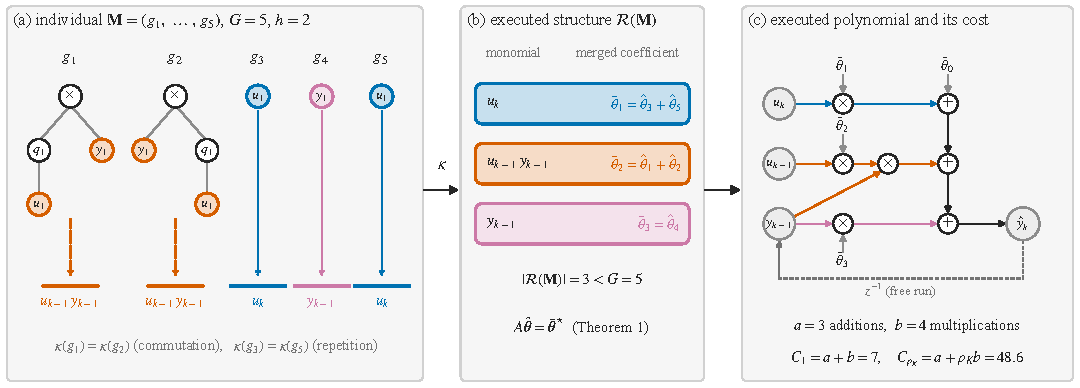
\includegraphics[width=\textwidth]{figures/fig_schematic.pdf}
\caption{From an individual to its arithmetic cost, for a model returned by Green MGGP on E1 ($\rho=1$, seed~13).
(a)~The five gene trees, with leaves coloured by the monomial that the gene denotes: $g_1$ and $g_2$ differ only by
commutation, and $g_3$ and $g_5$ coincide. (b)~The executed structure $\Rs(\M)$ has three monomials, and the
coefficients of genes with the same monomial are merged (Theorem~\ref{thm:invariance}). (c)~The executed polynomial,
simulated in free run, needs $a=3$ additions and $b=4$ multiplications per sample, so that $C_1=7$ and
$C_{\rho_K}=48.6$ in \eqref{eq:cost}. This illustrative model omits the true bilinear regressor and is not the generating structure.}
\label{fig:schematic}
\end{figure}

\subsection{Parameter estimation and structural invariance}
Let $N$ identification samples be given and let $\mathcal K=\{n+1,\dots,N\}$, where $n$ is the maximum delay of
the individual. The regression matrix $\Psi(\M)\in\R^{|\mathcal K|\times(G+1)}$ has a column of ones and the columns
$(\varphi_{\kappa(g_i)}(k))_{k\in\mathcal K}$, and $\bar\Psi(\Rs)\in\R^{|\mathcal K|\times(|\Rs|+1)}$ is the
corresponding matrix with one column per element of $\Rs$.

\begin{assumption}[Identifiability]\label{ass:rank}
$\bar\Psi(\Rs)$ has full column rank.
\end{assumption}

\begin{theorem}[Structural invariance of the identified model]\label{thm:invariance}
Let $\M$ be an individual with $\Rs=\Rs(\M)$ satisfying Assumption~\ref{ass:rank}, and let
$A\in\{0,1\}^{(|\Rs|+1)\times(G+1)}$ be the aggregation matrix with $A_{00}=1$ and $A_{mi}=1$ if and only if
$\kappa(g_i)=m$. Then:
\begin{enumerate}
\item[(i)] $\Psi(\M)=\bar\Psi(\Rs)A$;
\item[(ii)] every minimiser $\hat{\boldsymbol\theta}$ of $\|\mathbf y-\Psi(\M)\boldsymbol\theta\|_2$ satisfies
$A\hat{\boldsymbol\theta}=\bar{\boldsymbol\theta}^\star$, the unique minimiser of
$\|\mathbf y-\bar\Psi(\Rs)\bar{\boldsymbol\theta}\|_2$;
\item[(iii)] the identified model of $\M$ coincides with the model \eqref{eq:narx} of $\Rs$ with coefficients
$\bar{\boldsymbol\theta}^\star$. Consequently its one-step-ahead, multiple-shooting and free-run predictions, and
every objective computed from them, depend on $\M$ only through $\Rs(\M)$.
\end{enumerate}
\end{theorem}
\begin{proof}
(i) Column $i\ge1$ of $\Psi(\M)$ is the column of $\bar\Psi(\Rs)$ indexed by $\kappa(g_i)$, that is,
$\Psi e_i=\bar\Psi e_{\kappa(g_i)}=\bar\Psi Ae_i$; the constant columns agree because $A_{00}=1$.
(ii) Every row of $A$ contains a one, because every $m\in\Rs$ equals $\kappa(g_i)$ for some $i$, so $A$ is
surjective. Hence $\{\Psi\boldsymbol\theta\}=\{\bar\Psi A\boldsymbol\theta\}=\{\bar\Psi\bar{\boldsymbol\theta}\}$,
and the two least-squares problems have the same optimal value. If $\hat{\boldsymbol\theta}$ is a minimiser of the
first, $A\hat{\boldsymbol\theta}$ attains the optimal value of the second and is therefore a minimiser of it. Under
Assumption~\ref{ass:rank} the second objective is strictly convex, so its minimiser is unique.
(iii) For every argument,
$\hat\theta_0+\sum_{i=1}^{G}\hat\theta_i\varphi_{\kappa(g_i)}=\hat\theta_0+\sum_{m\in\Rs}\big(\sum_{i:\kappa(g_i)=m}\hat\theta_i\big)\varphi_m
=\theta^\star_0+\sum_{m\in\Rs}\theta^\star_m\varphi_m$. All three predictors evaluate this function recursively from
the data and from initial conditions of length $n(\Rs)$, which is itself a function of $\Rs$.
\end{proof}

\begin{corollary}\label{cor:classes}
Every objective that is a function of the identified model and of $\Rs(\M)$ is constant on the equivalence classes
of $\sim$. Removing all but one member of each class from a set of individuals therefore removes no objective vector.
\end{corollary}

\subsection{Error objective}
Multiple shooting limits simulation length by dividing the data into shorter segments~\cite{Ribeiro2020}. Here the package resets each segment to measured outputs; this windowed criterion does not include the optimised segment initial states and continuity constraints of the formulation in~\cite{Ribeiro2020}.

\begin{definition}[Multiple-shooting error]\label{def:je}
Let $n=n(\Rs(\M))$, $K\in\N$ and $W=\lfloor N/(n+K)\rfloor$. The identification samples are partitioned into $W$
disjoint windows of length $n+K$. In window $w$, the identified model is initialised with the $n$ measured outputs
and simulated in free run for $K$ steps, giving $\hat y_w(k)$. The error objective is
\begin{equation}
J_E(\M)=\frac{1}{\sigma_y}\left(\frac{1}{W(n+K)}\sum_{w=1}^{W}\sum_{k=1}^{n+K}\big(y_w(k)-\hat y_w(k)\big)^2\right)^{1/2},
\label{eq:je}
\end{equation}
where $\sigma_y$ is the standard deviation of the identification output, and $J_E(\M)=\infty$ if the estimation or
the simulation fails.
\end{definition}

The first $n$ residuals of each window vanish by construction. By Theorem~\ref{thm:invariance}, $J_E$ is a function
of $\Rs(\M)$. With $K=20$ it penalises the accumulation of error over a finite horizon at a fraction of the cost of a
full free-run simulation; the normalisation by $\sigma_y$ does not affect the search.

The definitions and structural-invariance results above describe the intended polynomial predictors. The unmodified package has a circular-buffer error in multiple shooting and free run: it retains only the maximum backshift in past outputs, so an output factor at that boundary can be evaluated as $y(k-1)$ instead of its intended delay. Least-squares estimation uses the intended delays. For affected individuals, the numerical error used by the search therefore differs from \eqref{eq:je} evaluated with the intended polynomial. All configurations retain this implementation, and the stored objectives are reported without correction. Input-only individuals without a backshift can be evaluated; the failure for no backshift concerns individuals containing output factors. These implementation restrictions qualify the empirical application of the ideal predictor definitions.

\subsection{Arithmetic-cost objective}

\begin{definition}[Arithmetic cost]\label{def:cost}
Evaluating \eqref{eq:narx} in direct form requires $a(\Rs)=|\Rs|$ additions and $b(\Rs)=\sum_{m\in\Rs}|m|$
multiplications, one for each coefficient and $|m|-1$ between the factors of each regressor. Let $\rho>0$ be the cost of
a multiplication relative to that of an addition on the platform that executes the model. In addition-equivalents, the
cost of a regressor and of an individual are
\begin{equation}
c_\rho(m)=1+\rho\,|m|,\qquad
C_\rho(\M)=\sum_{m\in\Rs(\M)}c_\rho(m)=a(\Rs)+\rho\,b(\Rs).
\label{eq:cost}
\end{equation}
Two weights are used. The bit-level weight of the Green-Box framework~\cite{NMN2023} charges $B$ bit
operations for an addition of $B$-bit operands and $B^{\alpha}$, $\alpha=\log_2 3$, for a Karatsuba multiplication~\cite{KO1963}; it corresponds to $\rho_K=B^{\alpha-1}$, which for binary64 operands ($B=64$) equals
$3^6/2^6=729/64\approx\rhoK$, and $B\,C_{\rho_K}=B\,a+B^{\alpha}b$ is the Green-Box complexity. The unit weight $\rho=1$
makes $C_1=a+b$ the number of arithmetic operations, which describes platforms on which both operations take
comparable time, such as processors with floating-point units; Section~\ref{sec:energy} shows that it is the weight
supported by the execution times measured in this study. We write $C$ for $C_\rho$ when the weight is clear.
\end{definition}

\subsubsection{Establishing the weights and separating the measurements}
The two declared scenarios are analysed throughout: $\rho=1$ is an unweighted operation count and $\rho_K=729/64$ is a theoretical bit-level weight. Neither is obtained from power measurements. The bit-level model does not describe the instruction-level cost of binary64 multiplication on this laptop. Operation counts are computed from each canonical structure before evaluation, independently of any measured runtime, energy or carbon intensity.

A platform-specific timing calibration instead estimates $\rho_{\mathrm{time}}=t_\times/t_+$ from $t=t_0+t_+a+t_\times b$. Here this fit characterises the Python simulator and includes interpreter overhead. Earlier timing measurements provide support for an order-one weight; they do not make $\rho=1$ an exact fitted value. In the corrected study both declared weights were fixed before the new searches. Subsequent timing checks assess those choices and cannot retrospectively redefine their objectives. A newly calibrated weight would require a separately declared search protocol. Section~\ref{sec:energy} separates timing, power integration and carbon conversion; its historical measurements are not measurements of the corrected models.

\begin{proposition}[Structure of the cost]\label{prop:cost}
Let $\rho>0$ and let $\Rs,\Rs'$ be structures of individuals in $\Gen_h^{\,G}$, with $D=2^h$:
\begin{enumerate}
\item[(i)] $C_\rho$ is modular: $C_\rho(\Rs\cup\Rs')=C_\rho(\Rs)+C_\rho(\Rs')-C_\rho(\Rs\cap\Rs')$;
\item[(ii)] $C_\rho$ is strictly monotone: $\Rs\subsetneq\Rs'$ implies $C_\rho(\Rs)<C_\rho(\Rs')$, and $|m|<|m'|$ implies $c_\rho(m)<c_\rho(m')$;
\item[(iii)] $(1+\rho)\,a(\Rs)\le C_\rho(\Rs)\le(1+\rho D)\,a(\Rs)$;
\item[(iv)] $C_\rho$ depends on $\Rs$ only through $(a,b)$, and the number of distinct values of $C_\rho$ over $\Gen_h^{\,G}$
is at most
\begin{equation}
L(G,h)=\sum_{a=1}^{G}\big(a(D-1)+1\big)=G+\frac{(D-1)G(G+1)}{2};
\label{eq:levels}
\end{equation}
\item[(v)] for $\rho=\rho_K$ and $G<729$, the map $(a,b)\mapsto C_{\rho}$ is injective, so the cost determines both the
number of terms and the total degree; for $\rho=1$ it is not, and $C_1$ takes at most $G(D+1)-1$ values.
\end{enumerate}
\end{proposition}
\begin{proof}
(i) $C_\rho$ is a sum of $c_\rho$ over the elements of a set. (ii) $c_\rho(m)>0$ for every $m$, and $c_\rho$ is strictly
increasing in $|m|$. (iii) By Lemma~\ref{lem:kappa}(c), $1\le|m|\le D$. (iv) The first statement is
\eqref{eq:cost}; moreover $a\in\{1,\dots,G\}$ and, by (iii), $a\le b\le aD$, which gives at most $a(D-1)+1$ values of $b$
for each $a$. (v) $\rho_K=64^{\log_2 3-1}=3^6/2^6$. If $a+\rho_K b=a'+\rho_K b'$, then $64(a-a')=729(b'-b)$; since
$\gcd(64,729)=1$, $729$ divides $a-a'$, and $|a-a'|<G<729$ forces $a=a'$ and then $b=b'$. For $\rho=1$,
$(a,b)=(2,2)$ and $(1,3)$ have the same cost, and $C_1=a+b$ ranges over the integers from $2$ to $G(D+1)$.
\end{proof}

\begin{remark}
The complexity used in the tutorial of the package, $\omega$ times the number of \texttt{mul} nodes, assigns
$c_\omega(m)=\omega(|m|-1)$ to each gene and sums over genes rather than over $\Rs(\M)$. It violates
Proposition~\ref{prop:cost}(ii), because a linear regressor costs nothing, so adding linear terms never increases the
cost, and it charges duplicated genes that are executed once.
\end{remark}

\begin{proposition}[Invariance to monotone rescaling]\label{prop:rescaling}
Let $\psi:\R\to\R$ be strictly increasing. The Pareto order and the lexicographic order induced by $(J_E,\psi\circ C)$
coincide with those induced by $(J_E,C)$. In particular, any constant factor $\omega>0$ applied to a cost has no effect
on an algorithm whose decisions depend only on these orders, and the Green-Box complexity $B\,C_{\rho_K}$ induces the
same orders as $C_{\rho_K}$.
\end{proposition}
\begin{proof}
$\psi$ preserves $\le$, $<$ and $=$, and both orders are defined from these relations applied componentwise.
\end{proof}

The weight $\rho$, in contrast, is not a rescaling: it changes the relative cost of structures with different numbers of
terms and degrees, and hence the orders. A structure with fewer, higher-degree terms can be cheaper than one with more,
linear terms under $\rho=1$ and more expensive under $\rho_K$, so the weight must reflect the target platform.

\subsection{Bi-objective problem}
We use Pareto dominance to compare the objectives and hypervolume to measure the dominated region~\cite{ZT1999}.

\begin{definition}[Dominance, Pareto set, hypervolume]\label{def:pareto}
For $\F=(J_E,C)$, $\M$ dominates $\M'$, written $\M\prec\M'$, if $\F(\M)\le\F(\M')$ componentwise and
$\F(\M)\ne\F(\M')$. For a finite set $P$, $\ND(P)$ is its subset of non-dominated elements. The problem is
\begin{equation}
\min_{\M\in\Gen_h^{\,G}}\ \F(\M)=\big(J_E(\M),\,C(\M)\big),
\label{eq:mop}
\end{equation}
whose solution is the set of non-dominated individuals. For a reference point $\mathbf r$, the hypervolume of $P$
is the Lebesgue measure $\HV(P)=\lambda\big(\bigcup_{\M\in P}[\F(\M),\mathbf r]\big)$.
\end{definition}

If every element of $P$ is weakly dominated by an element of $Q$, then the region dominated by $P$ is contained in
that dominated by $Q$, so $\HV(P)\le\HV(Q)$; this monotonicity is used below.

\subsection{Selection schemes}
Both schemes share one generation template: parent selection by binary tournament, crossover and mutation with the
operators of the package, least-squares estimation and evaluation of the modified offspring, and elitist survival.
They differ only in the relation used to compare individuals and in the survival rule.

\paragraph{Lexicographic scheme (MO-lex).}
In the bi-objective mode of the package~\cite{mggpy}, tournaments and the hall of fame use DEAP fitness comparisons~\cite{FDG+2012,DEAPFitness}, which follow the
lexicographic order: $\F(\M)<_{\mathrm{lex}}\F(\M')$ if $J_E(\M)<J_E(\M')$, or $J_E(\M)=J_E(\M')$ and $C(\M)<C(\M')$.
The single-objective configuration (SO) compares $J_E$ only. The run returns $\ND(P_T)$ in MO-lex and the best
individual in SO, where $P_T$ is the final population.

\begin{theorem}[Lexicographic reduction]\label{thm:lex}
Run SO and MO-lex from the same initial population with the same pseudo-random stream. Suppose that, up to generation
$t$, every pair of individuals compared by a tournament or by the hall of fame with $J_E(\M)=J_E(\M')$ also satisfies
$C(\M)=C(\M')$. Then both runs produce the same populations $P_0,\dots,P_t$. If the condition holds for all
generations, MO-lex returns $\ND(P_T^{\mathrm{SO}})$, the non-dominated subset of the final SO population.
\end{theorem}
\begin{proof}
By induction on the generation. $P_0$ is common. Suppose that $P_s$ is common. A generation is a deterministic
function of the current population, of the pseudo-random numbers it consumes and of the outcomes of the comparisons it
performs; the number and order of the random draws depend only on the population and on these outcomes. For a
compared pair with $J_E(\M)\ne J_E(\M')$, both relations order the pair as $J_E$ does. For a pair with
$J_E(\M)=J_E(\M')$, the hypothesis gives $C(\M)=C(\M')$, so both relations declare a tie, which the implementation
resolves by position in the same way. All outcomes coincide, the same random numbers are consumed, the same offspring
are produced and evaluated deterministically, and $P_{s+1}$ is common. The adaptation of the mutation rate depends
on $J_E$ of the best individual and is therefore also common. The last statement follows from $P_T^{\mathrm{lex}}=P_T^{\mathrm{SO}}$.
\end{proof}

Theorem~\ref{thm:lex} states that the lexicographic scheme is the single-objective algorithm followed by a
non-dominated filter, unless exact ties in $J_E$ between individuals with different costs occur. Since $J_E$ is a
continuous function of the data, such ties essentially arise only among individuals whose estimation or simulation
fails ($J_E=\infty$); Section~\ref{sec:results} verifies the theorem empirically.

\paragraph{Pareto-based scheme (Green MGGP).}
Green MGGP replaces the comparison relation and the survival rule by those of NSGA-II~\cite{DPAM2002}.

\begin{definition}[Rank and crowding]\label{def:crowding}
For a finite set $P$, let $\mathcal F_1=\ND(P)$ and $\mathcal F_{r+1}=\ND(P\setminus\bigcup_{s\le r}\mathcal F_s)$.
The rank of $\M\in\mathcal F_r$ is $r$, and its crowding distance is
\begin{equation}
\delta(\M)=\sum_{i=1}^{2}\frac{F_i(\M^{+}_i)-F_i(\M^{-}_i)}{F_i^{\max}-F_i^{\min}},
\label{eq:crowding}
\end{equation}
where $\M^{\pm}_i$ are the neighbours of $\M$ in $\mathcal F_r$ sorted by $F_i$, the extremes and normalisation are
taken over $\mathcal F_r$, and boundary elements receive $\delta=\infty$. The crowded order prefers lower rank and,
for equal ranks, larger $\delta$.
\end{definition}

\begin{algorithm}[t]
\caption{One generation of Green MGGP}\label{alg:green}
\begin{algorithmic}[1]
\Require population $P_t$ with $|P_t|=\mu$; crossover and mutation rates $p_c$, $p_m$
\State assign rank and crowding distance \eqref{eq:crowding} to all $\M\in P_t$
\State $Q_t\gets$ $\mu$ copies selected by binary tournament under the crowded order
\State apply package crossover to consecutive pairs of $Q_t$ with probability $p_c$
\State apply package mutation to each $\M\in Q_t$ with probability $p_m$
\State estimate $\hat{\boldsymbol\theta}$ and evaluate $\F$ for every modified individual
\State $U_t\gets$ one representative per class of $\sim$ among the elements of $P_t\cup Q_t$ with finite $\F$
\State $P_{t+1}\gets$ the first $\mu$ elements of $U_t$ under the crowded order (NSGA-II truncation); if $|U_t|<\mu$,
complete with the remaining individuals
\end{algorithmic}
\end{algorithm}

\begin{theorem}[Non-deterioration of the population front]\label{thm:elitism}
Let $U_t^1=\ND(U_t)$ in Algorithm~\ref{alg:green} and suppose that $P_t$ contains an individual with finite $\F$.
If $|U_t^1|\le\mu$, then:
\begin{enumerate}
\item[(i)] $U_t^1\subseteq P_{t+1}$;
\item[(ii)] for every $\M\in\ND(P_t)$ there is $\M'\in\ND(P_{t+1})$ with $\F(\M')\le\F(\M)$;
\item[(iii)] $\HV(\ND(P_{t+1}))\ge\HV(\ND(P_t))$ for every reference point.
\end{enumerate}
Moreover, if no two elements of $U_t^1$ share an objective vector, then $|U_t^1|\le L(G,h)$ in \eqref{eq:levels},
so $L(G,h)\le\mu$ is a sufficient condition for (i)--(iii) at every generation.
\end{theorem}
\begin{proof}
(i) NSGA-II truncation admits the fronts of $U_t$ in increasing rank, and $\mathcal F_1=U_t^1$ fits entirely.
(ii) Let $\M\in\ND(P_t)$. Since $P_t$ has an element with finite $\F$, so does $\M$. Its class has a representative
$\tilde\M\in U_t$ with $\F(\tilde\M)=\F(\M)$ (Corollary~\ref{cor:classes}). Because $U_t$ is finite and $\prec$ is a
strict partial order, either $\tilde\M\in U_t^1$ or some $\M'\in U_t^1$ dominates $\tilde\M$; in both cases there is
$\M'\in U_t^1$ with $\F(\M')\le\F(\M)$, and $\M'\in P_{t+1}$ by (i). Every element of $P_{t+1}$ either belongs to
$U_t$, shares its objective vector with an element of $U_t$, or has $\F=(\infty,\infty)$; none of them dominates
$\M'$, so $\M'\in\ND(P_{t+1})$.
(iii) follows from (ii) and the monotonicity of the hypervolume.
For the bound, two elements of a non-dominated set with the same cost must have the same error, since otherwise one
dominates the other; when no two elements share an objective vector, $U_t^1$ has at most one element per value of $C_\rho$,
and Proposition~\ref{prop:cost}(iv) bounds the number of these values by $L(G,h)$ for every $\rho>0$.
\end{proof}

The single-objective and lexicographic schemes enjoy no such guarantee for the cost dimension: their elitism retains
the individuals with the lowest $J_E$, so a cheap non-dominated individual can be lost from one generation to the next.

\subsection{Selecting a single model}

\begin{definition}[$\tau$-rule]\label{def:tau}
For a returned set $P$, $\tau\ge0$ and $\eta\ge0$, let $J^{\min}=\min_{\M\in P}J_E(\M)$ and
\begin{equation}
\mathcal M_\tau\in\arg\min\big\{\,C(\M):\ \M\in P,\ J_E(\M)\le(1+\tau)J^{\min}+\eta\,\big\},
\label{eq:tau}
\end{equation}
with ties broken by the smaller $J_E$.
\end{definition}

\begin{proposition}[Properties of the $\tau$-rule]\label{prop:tau}
(i) $\mathcal M_\tau\in\ND(P)$. (ii) $\tau\mapsto C(\mathcal M_\tau)$ is non-increasing; if $P=\ND(P)$, then
$\tau\mapsto J_E(\mathcal M_\tau)$ is non-decreasing. (iii) $\mathcal M_0$ is the cheapest model of minimal error up
to $\eta$, and for $\tau$ large enough $\mathcal M_\tau$ is the cheapest model in $P$.
\end{proposition}
\begin{proof}
(i) Suppose $\M\prec\mathcal M_\tau$. Then $J_E(\M)\le J_E(\mathcal M_\tau)$, so $\M$ is feasible, and
$C(\M)\le C(\mathcal M_\tau)$. Minimality of the cost forces $C(\M)=C(\mathcal M_\tau)$, and then
$J_E(\M)<J_E(\mathcal M_\tau)$ contradicts the tie-breaking rule. (ii) The feasible set grows with $\tau$, so its
minimum cost cannot increase. If $P$ is non-dominated, a smaller cost implies a larger error, and an equal cost
implies an equal vector. (iii) is immediate from the definition.
\end{proof}

We use $\tau=\tauSel$ and $\eta=10^{-6}$, fixed before the experiments; $\mathcal M_\tau$ is then the cheapest model
whose identification error lies within $5\%$ of the best error found, and $\eta$ only matters on noise-free data,
where the best error is at machine precision. For SO, $P$ contains a single model. The rule uses identification
data only, and its sensitivity to $\tau$ is examined in Section~\ref{sec:results}.
